\documentclass[utf8x, 12pt]{G7-32} % Стиль (по умолчанию будет 14pt)

% Остальные стандартные настройки убраны в preamble.inc.tex.
\include{00-preamble.inc}

\ifPDFTeX
\include{00-listings.inc}
\else
\usepackage{local-minted} % Настройки листингов.
\fi
\include{00-macros.inc} % Полезные макросы листингов.

\begin{document}
\frontmatter
\thispagestyle{empty} % Отключение нумерации страницы.
\begin{center}
Федеральное государственное бюджетное образовательное учреждение
высшего профессионального образования \\

%\begin{figure}
%\begin{minipage}[h]{0.49\linewidth}
%\includegraphics[width=0.5\linewidth]{title/bmstu_emblem} 
%\end{minipage}
%\hfill
%\label{ris:emblem}
%\end{figure}
\textbf{«Московский государственный технический университет имени Н.Э. Баумана»}
\textbf{(МГТУ им. Н.Э. Баумана)}

\hrulefill

\begin{flushleft}
ФАКУЛЬТЕТ: Информатика и системы управления \\
КАФЕДРА: Программное обеспечение ЭВМ и информационные технологии \\
\end{flushleft}

\vspace{4cm}
\textbf{РАСЧЕТНО-ПОЯСНИТЕЛЬНАЯ ЗАПИСКА} \\
\textbf{к курсовой работе на тему:} \\
\vspace{0,5cm}
Разработка программного обеспечения для управления мышью с помощью Android-устройства для операционной системы "Linux".
\end{center}
\vspace{8cm}
\begin{flushright}
\textbf{Руководитель курсовой работы} \makebox[3cm]{\hrulefill} /Оленев А.А./ \\
\vspace{0,2cm}
\textbf{Студент} \makebox[3cm]{\hrulefill} /Кукуев С.А./
\end{flushright}
\vspace{1cm}
\begin{center}
Москва, 2016.
\end{center}

%%% Local Variables: debug
%%% mode: latex
%%% TeX-master: "rpz-os"
%%% End:
\tableofcontents % автоматическая генерация содержания
\chapter{Введение}
\label{cha: intro}
	Сегодня сложно представить себе работу с персональным компьютером без привычного каждому из нас устройства - мыши. С момента создания этот девайс претерпел колоссальные изменения. От обычных механических мышей, с которыми было неудобно работать в виду тяжелого веса и плохого позиционирования, мир перешел к оптическим, отличавшимся легкостью, надежностью и высокой точностью. Несмотря на это, метаморфозы устройства продолжаются. В настоящее время появились гироскопические мыши\cite{gyrmouse}, позволяющее распознавать движение не только на поверхности, но и в пространстве. Для тех, кто использует большие плазменные экраны или проекторы, такое новшество позволяет управлять компьютером в качестве пульта, не задействуя посторонние предметы. Но стоимость таких мышей составляет порядка 4-5 тысячи рублей, что в свою очередь является дорогим удовольствием.
	
\label{txt: tasks} 
% Из задач должно быть понятно, что я хочу сделать в курсовом проекте. Необходимо конкретезировать каждую задачу и иметь для нее ощутимую метрику. (Добавить точные цифры к требованиям)
	Данное программное обеспечение позволяет использовать Android-устройство в качестве беспроводной мыши и выполнять соответствующую функциональность. В процессе реализации должны быть решены следующие задачи:
\begin{itemize}
\item Задержка обработки данных.
	Программное обеспечение обрабатывает данные в реальном времени. При таком подходе важно учесть скорость передачи данных и их последующую обработку. Поскольку передается небольшой объем данных, со скоростью не должно возникнуть проблем, а вот слишком большая задержка увеличит дергание курсора.
\item Дрожание мыши.
	Для реализации используются датчики Android-устройства, погрешность которых достигает порядка 5° (в зависимости от выбора датчика). Помимо того, использование акселерометра или гироскопа добавляет внешний фактор - дрожание человеческой руки. Все это в совокупности вызывает дребезжание курсора, которое необходимо минимизировать.
\item Функциональность.
	Под функциональностью понимается минимальный набор требуемых функций, необходимых для замены базовой мыши. В данном случае будет достаточно поддержки двух осей вращения и двух кнопок.
\end{itemize}

%%% Local Variables: debug
%%% mode: latex
%%% TeX-master: "rpz-os"
%%% End
\mainmatter % начало нумерации
\chapter{Аналитический раздел}
\label{cha:analysis}
	Перед проведением анализа необходимо разбить реализацию на независимые части. Для каждой предстоит выбрать алгоритм, удовлетворяющий поставленным задачам. Проанализировав возможные методы реализации были выделены следующие подсистемы:
\begin{itemize}
\item Способы управления курсором.
\item Передача данных с Android-устройства.
\item Обработка полученных данных.
\item Взаимодействие с ядром.
\end{itemize}
\begin{figure}
  \centering
  \includegraphics[scale=0.75]{analysis/structure}
  \caption{Общая структура.}
  \label{fig: view_arch}
\end{figure}
\label{sec: gyro&accel}
\section{Выбор способа управления}
	Для выбора способа управления необходимо отталкиваться от поставленных задач. Самый распространенный вариант - имитация сенсорной панели. При такой реализации дрожание курсора зависит лишь от задержки обработки данных. С другой стороны, присутствие в Android-устройствах таких датчиков\cite{gyr&accel}, как G-сенсор и гироскоп, дают дополнительную степень свободы, что позволяет получить большую функциональность.
	
	Гироскоп (гиродатчик) - устройство, позволяющее определить ориентацию в пространстве, используя гравитацию Земли. По количеству степеней свободы различают: двухстепенные и трехстепенные. На Android устройствах на сегодняшний день установлены вибрачионные микрогироскопы, принцип действия которых основан на силе Кориолиса\cite{coriolis}. 
	
	Акселерометр (G-сенсор) - устройство, предназначенное для измерения негравитационного ускорения. Различают три типа: однокомпонентные, двухкомпонентные и трехкомпонентные. Чтобы определить ориентацию в пространстве, необходимо данные измерения проинтегрировать, получая инерциальную скорость и координаты устройства. 

	Основным из преимуществ гироскопа является то, что акселерометр не в состоянии отличить гравитационное ускорение от любого другого. Находясь в системе отсчета, которая ускорено движется в определенном направлении, данный датчик будет показывать некорректные результаты. Гироскопы в свою очередь ориентируются лишь на гравитацию и не зависят от внешних факторов, поэтому и были выбраны в качестве способа управления.
\label{sec: bt&wifi}
\section{Методы передачи данных}
	Взаимодействие Android-устройства и персонального компьютера является необходимой частью реализации, поэтому необходимо выбрать один из существующих методов. Основными факторами выбора будут: радиус действия, скорость передачи и сложность настройки. Вариант с USB 3.0, не смотря на высокую скорость, не подходит из-за наличия проводной передачи данных.
	
	Bluetooth и wi-fi\cite{bt&wifi} являются беспроводными стандартами связи и используют для передачи данных определенные радиочастоты. Чтобы определиться с выбором метода, составим таблицу из самых распространенных стандартов с данными о радиусах действия и максимальных скоростях передач.
\begin{center}
\begin{table}[h]
  \caption{Сравнение стандартов}
  \begin{tabular}{|r|c|c|}
 	\hline
    Стандарт 		& Дистанция(в помещении), m & Скорость, Mbps \\
    \hline
    Wi-fi			&                	 		&              	 \\
    \hline
	IEEE 802.11.g   & 			38 		   		&    	54     	 \\
    IEEE 802.11.n   & 			70		   		&      600     	 \\
    \hline
    Bluetooth		&					   		&				 \\
    \hline
    Bluetooth 3.0	&			10		   		&		24		 \\
    Bluetooth 4.0	&			60	 	   		&		30 		 \\
    \hline
  \end{tabular}
  \label{tabl: bt&wifi}
\end{table}
\end{center}

	В таблице~\ref{tabl: bt&wifi} наглядно видно, что wi-fi обладает лучшими характеристиками. Но для передачи информации он требует тщательной настройки параметров, а также обязательного наличия третьего звена - точки-маршрутизатора. Возможен вариант соединения ad-hoc, который позволяет соединяться напрямую, но при этом станет невозможно подключить другие устройства. Bluetooth же не требует никакого дополнительного конфигурирования и позволяет подключить несколько устройств одновременно. Для передачи координат с Android-устройства хватает скорости передачи и bluetooth, поэтому он выбран для реализации передачи информации.

\label{sec: int_event}	
\section{Интерфейсы событий}
	В операционной системе Linux для решения поставленной задачи существует специальная подсистема ввода ядра\cite{ldd3}, которая объединяет все рассеянные драйвера для обработки перифирийных устройств. Одним из ее плюсов является удобный интерфейс событий, позволяющий драйверу не создавать и не управлять узлами /dev и связанными с ними методами доступа. Вместо этого он имеет возможность вызывать API для ввода, чтобы отправить движения мыши. Такие системы, как X Window, хорошо взаимодействуют с интерфейсами событий, экспортируемыми подсистемой ввода. 

	Чтобы выбрать один из возможных интерфейсов, необходимо обозначить требования, которым он должен соответствовать, и ознакомиться со всеми доступными вариантами. Исходя из задач, поставленных в рамках реализации, основным требованием к интерфейсу является необходимая функциональность. Кроме движения мыши, драйвер событий должен предоставлять возможность нажатия на кнопки мыши. Рассмотрим три возможных варианта: evdev, mousedev и собственный интерфейс.

	<<\verb|Evdev|>> - универсальный драйвер событий ввода. Каждый пакет события, создаваемый <<\verb|evdev|>>, имеет строго определенный формат и содержит в себе следующие параметры: время, тип события, код события, значение события. Одно из преимуществ интерфейса является простота использования и универсальность. Кроме того, он имеет возможность работать с акселерометром, что упростит задачу преобразования данных, и оснащен минимальным требуемым функционалом для решения задачи.

	<<\verb|Mousedev|>> - специальный драйвер событий ввода для мыши. В отличие от универсального evdev, этот интерфейс предназначен лишь для одного перефирийного устройства, и не умеет взаимодействовать с такими датчиками, как гироскоп и акселерометр. Функций у драйвера намного больше.

	Помимо готовых вариантов, имеется возможность написать собственный драйвер событий. Является более гибким вариантом, чем два, представленных выше, поскольку мы сможем постепенно наращивать функционал.

	Для решения поставленной задачи целесообразней использовать универсальный драйвер событий ввода. Поскольку он оснащен требуемой функциональностью, и прост в использовании.
	
%%% Local Variables: debug
%%% mode: latex
%%% TeX-master: "rpz-os"
%%% End:
\chapter{Конструкторский раздел}
\label{design}
\section{Структура разрабатываемого программного обеспечения}
	Для создания разрабатываемого программного обеспечения необходимо реализовать:
\begin{itemize}
\item Загружаемый модуль ядра.
\item Пользовательское приложение.
\end{itemize}

	Согласно поставленной задачи, пользователь должен осуществлять управление мышью через Android устройство удаленно, поэтому пользовательское приложение необходимо реализовать в виде клиент-серверного приложения. Таким образом, пользовательское приложение будет состоять из двух частей: программы сервера и программы клиента.
\begin{itemize}
\item Клиент - приложение, разработанное для Android устройства, которое предоставляет ползователю осуществлять управление мышью.
\item Сервер - приложение, работающее на ПК в фоновом режиме, отвечающее за получение данных от клиентского приложения и передачу их загружаемому модулю ядра.
\end{itemize}

	Передача данных между смартфоном и ПК будет осуществляться с помощью протокола RFCOMM\cite{btprotocol}. Используется как транспортный протокол протоколом L2CAP\cite{btprotocol} (базовый протокол передачи данных для Bluetooth). Основной принцип действия заключается в эмулировании соединения point-to-point по последовательному порту. В связи с этим, структура программного обеспечения будет выглядеть как на рисунке~\ref{fig: view_struct}.
\begin{figure} [h!]
  \centering
  \includegraphics[scale=0.75]{design/structure}
  \caption{Структура программного обеспечения}
  \label{fig: view_struct}
\end{figure}
\label{sec: format}
\section{Формат передаваемых данных между приложениями}
	При обмене информацией между всеми приложениями необходимо определить содержание и формат передаваемых данных. Для корректной работы мыши, загружаемый модуль должен получать текущие координаты положения курсора и тип команды. Передаваемые данные запишем в виде строки, представленной на рисунке~\ref{fig: format}, состоящей из 4 чисел:
\begin{figure} [h!]
  \centering
  \includegraphics[scale=1]{design/format}
  \caption{Формат передаваемых данных}
  \label{fig: format}
\end{figure}

	Также, необходимо сразу уточнить, какие команды могут подаваться от устройства:
\begin{itemize}
\item Перемещение курсора
\item Нажатие левой клавиши мыши
\item Нажатие правой клавиши мыши
\item Двойной щелчок левой клавиши мыши
\end{itemize}
\label{sec: android}
\section{Приложение для Android устройства}
	Клиентское приложение уровня пользователя должно осуществлять обработку датчиков устройства, обработку запросов пользователя, установку соединения с серверным приложением и последующую передачу данных.

\paragraph{Работа с датчиками Android устройства}
	
	В качестве способа управления был выбран гироскоп. В Android устройстве он представлен двумя структурами\cite{sensor}: \Code{TYPE\_GYROSCOPE} и \Code{TYPE\_GYROSCOPE\_UNCALIBRATED}. Отличия структур в том, что \Code{TYPE\_GYROSCOPE\_UNCALIBRATED} хранит скорости вращения вокруг осей X, Y и Z без дрейфa датчика, тем самым данные скорости являются неоткалиброваными. При этом дрейф содержится в отдельных переменных. Для данного программного обеспечения была выбрана структура откалиброванного гироскопа (\Code{TYPE\_GYROSCOPE}).
	
	Чтобы начать работу с датчиком, необходимо его проинициализировать:
\begin{lstlisting}[style=pseudocode,caption={Инициализация датчика}]
	SensorManager := (SensorManager) getSystemService(Context.SENSOR_SERVICE);
	Sensor := SensorManager.getDefaultSensor(Sensor.TYPE_GYROSCOPE);
\end{lstlisting}

	После инициализации выставляем интервал получения данных от гироскопа и сохраняем информацию, полученную от датчика:
\begin{lstlisting}[style=pseudocode,caption={Установка времени и функция сохранения данных}]
	sensorManager.registerListener(listener, sensorGyro, SensorManager.SENSOR_DELAY_NORMAL)
						...
	dev getData(SensorEvent event):
		for (int i=0; i < 3; i++)	
			valuesGyro[i] = event.values[i]
\end{lstlisting}	 
\paragraph{Работа с Bluetooth}
 
	Для установки соединения с сервером необходимо использовать Bluetooth API~\cite{btandroid}. Работа с bluetooth происходит в 4 этапа:
\begin{enumerate}
\item Инициализация адаптера.
\item Поиск доступного сервера.
\item Установка соединения.
\item Передача данных.
\end{enumerate} 

	Инициализация адаптера происходит с помощью функции \Code{BluetoothAdapter.getDefaultAdapter()}. Передача данных осуществляется при помощи сокетов. Сокет - это название программного интерфейса для обеспечения обмена данными между процессами\cite{socket}. Процессы при таком обмене могут исполняться как на одной ЭВМ, так и на различных ЭВМ, связанных между собой сетью. Сокет — абстрактный объект, представляющий конечную точку соединения. Ниже представлен алгоритм подключения к серверу:
\begin{lstlisting}[style=pseudocode,caption={Алгоритм подключения к серверу}]
def connectToServer():
	device := adapter.getRemoteDevice(SERVER_MAC_address)
	socket := device.createRfcommSocketToServiceRecord(SERVER_UUID)
	adapter.cancelDiscovery()
    socket.connect()
	stream := socket.getOutputStream()
\end{lstlisting}
	Для передачи данных мы используем выходной поток \Code{stream}, созданный при подключении.
\begin{lstlisting}[style=pseudocode,caption={Алгоритм передачи данных}]
def sendDataToServer(command, coordinates):
	msg := Integer.toString(command) + " " +
                Integer.toString(coordinates[0]) + " " +
                Integer.toString(coordinates[1]) + " " +
                Integer.toString(coordinates[2]) + "\n"
	buffer := msg.getBytes()
	if (stream != null)
		stream.write(buffer)
\end{lstlisting}
\label{sec: server}
\section{Серверное приложение}
	Серверное приложение уровня пользователя должно решать следующие задачи:
\begin{itemize}
\item Установка соединения с клиентским приложением.
\item Получение данных от клиентского приложения.
\item Передача данных в пространство ядра.
\end{itemize}
	Установка соединения с клиентским приложением осуществляется по алгоритму 2.1. Перед запуском сервера~\cite{bluez} необходимо установить уникальный UUID - 16-байтный номер, используемый для уникальной идентификации сервера. Кроме того, требуется установить значение порта.  
\begin{lstlisting}[style=pseudocode,caption={Алгоритм запуска сервера}]
def startServer():
	server.socket := BluetoothSocket(RFCOMM)
	server.socket := bind("",server.port)
	server.socket := listen(server.port)
	
    advertise_service( server.socket, server.name, 
    	service_id := server.uuid,
		service_classes := [ server.uuid, SERIAL_PORT_CLASS ],
		profiles = [ SERIAL_PORT_PROFILE ]
		)
		
	print("Waiting a client...")
	
	client.socket, client.info := server.socket := accept()
\end{lstlisting}

	После запуска, сервер находится в ожидании подключения клиента. Как только один из клиентов подал правильный sdp-запрос, сервер переходит в бесконечный цикл для приема данных от клиента и последующей записи в пространство ядра. 
\begin{lstlisting}[style=pseudocode,caption={Алгоритм передачи данных в пространство ядра}]
def sendData():
	while True:
        data := client.socket := recv(size)
        if len(data) == 0: break
        os.write(fd, data) # fd - file created by the driver for the adoption of the coordinates
        os.fsync(fd)
        if "</EOM>" in data: break
\end{lstlisting}

	Как только клиент отправил запрос об окончании передачи данных, сервер отправляет ответное сообщение о закрытии подключения и закрывает сначала клиентский сокет, а затем и свой.
\begin{lstlisting}[style=pseudocode,caption={Закрытие подключения}]
def stopServer():
	client.socket := send("The server will be turned off soon")

	client.socket := close()
	server.socket := close()
\end{lstlisting}
\label{sec: driver}
\section{Загружаемый модуль ядра}
	Загружаемый модуль ядра должен решать следующие задачи:
\begin{itemize}
\item Чтение данных из пространства ядра.
\item Регистрация устройства в подсистеме ввода ядра.
\end{itemize}
\paragraph{Чтение данных из пространства ядра}

	Обмен данными между пространством ядра и пространством пользователя происходит при помощи виртуальной файловой системы в ОС Linux - \texttt{sysfs}\cite{ldd3}. В \texttt{sysfs} имеется подкаталог, где содержится вся информация о перифирийных подключаемых устройствах, присущих конкретной платформе. Все, что необходимо для обмена: создать в этом самом подкаталоге \texttt{/sys/devices/platform}, каталог с файлом, в который сервер будет записывать поступающие данные от Android приложения. Данный каталог создается командой \Code{command\_result = sysfs\_create\_group(\&vms\_dev->dev.kobj, \&vms\_attr\_group);}.
	
\paragraph{Регистрация устройства в подсистеме ввода ядра}

Регистрация устройства происходит по следующим этапам:
\begin{enumerate}
\item Регистрация платформо зависимого устройства в системе.
\item Создание файла устройства в \Code{sysfs}.
\item Выделение памяти под устройство ввода.
\item Установка обработчика на события.
\item Регистрация устройства в подсистеме ввода.
\end{enumerate}
\begin{lstlisting}[style=pseudocode,caption={Алгоритм регистрации устройства в системе}]
def display_init(void):
    command_result = 0;

    vms_dev := platform_device_register_simple("vms", -1, NULL, 0)
    if (IS_ERR(vms_dev)) 
        PTR_ERR(vms_dev)
        printk("vms_init: error\n")
        return ERROR_REGISTER_PLATFORM_DEVICE

    command_result := sysfs_create_group(vms_dev->dev.kobj, vms_attr_group);
    
    if (command_result < 0)
        printk("Error sysfs_create_group\n")
        return ERROR_SYSFS_CREATE_GROUP

    vms_input_dev := input_allocate_device()
    if (!vms_input_dev) 
        printk("Bad input_alloc_device()\n")
        return ERROR_ALLOCATE_INPUT_DEVICE

    set_bit(EV_REL, vms_input_dev->evbit)
    set_bit(REL_X, vms_input_dev->relbit)
    set_bit(REL_Y, vms_input_dev->relbit)
    set_bit(EV_KEY, vms_input_dev->evbit)
    set_bit(BTN_LEFT, vms_input_dev->keybit)
    set_bit(BTN_RIGHT, vms_input_dev->keybit)

    vms_input_dev->evbit[0] := BIT_MASK(EV_KEY) | BIT_MASK(EV_REL)
    vms_input_dev->keybit[BIT_WORD(BTN_MOUSE)] := BIT_MASK(BTN_LEFT) |
        BIT_MASK(BTN_MIDDLE) | BIT_MASK(BTN_RIGHT)
    vms_input_dev->relbit[0] := BIT_MASK(REL_X) | BIT_MASK(REL_Y)

    vms_input_dev->name := "Virtual BT mouse"
    vms_input_dev->id.bustype := BUS_VIRTUAL
    vms_input_dev->id.vendor  := 0x0000
    vms_input_dev->id.product := 0x0000
    vms_input_dev->id.version := 0x0000
    
    command_result := input_register_device(vms_input_dev)
    
    if (command_result < 0)
        printk("Error input_register_device\n")
        return ERROR_REGISTER_INPUT_DEVICE
  
    printk("Virtual BT Mouse Driver Initialized.\n")
    return 0
\end{lstlisting}

%%% Local Variables: debug
%%% mode: latex
%%% TeX-master: "rpz-os"
%%% End:
\chapter{Технологический раздел}
\label{cha: impl}
\label{sec: lang}
\section{Выбор языка программирования}
	Комплекс программ разработан для использования в операционной системе Linux Ubuntu. В рамках реализации было разработано три программы:
\begin{itemize}
\item Драйвер устройства.
\item Bluetooth сервер.
\item Пользовательское приложение для Android устройства.
\end{itemize}
	Драйвер устройства для Linux разработан на языке Си. Данный выбор ограничен внутренним устройством ОС Linux и отсутствием средств разработки с использованием других языков.
	
	Bluetooth сервер для приема данных разработан на языке Python. Выбор основан на простоте использования rfcomm сокетов с использованием протокола sdp.
	
	Пользовательское приложение на платформе Android разработано на Java. Данный язык имеет строгую статическую типизацию, за счет чего выигрывает в производительности.
\label{sec: enviroment}
\section{Выбор среды программирования}
	Для драйвера устройства и bluetooth сервера было решено использовать стандартный текстовый редактор и соответствующие компиляторы для языков: C и Python - gcc и python. В качестве средства разработки был выбран Sublime Text 2 - текстовый редактор с подцветкой синтаксиса. Приложение под Android разрабатывалось в интегрированной среде разработке Android Studio. Выбор был сделан в пользу данной IDE, поскольку Eclipse прекратила поддержку плагина Android Development Tools(ADP) в 2014 году. Из плюсов необходимо выделить:
\begin{itemize}
\item Способность протестирвать приложение на устройствах с разным экраном и с разной версией API.
\item Множество шаблонов и макетов компонентов Android.
\end{itemize}
\label{sec: set&use}
\section{Установка и использование программного обеспечения}
	Для корректной работы драйвера и Android приложения необходимо скомпилировать модуль с помощью make файла и положить его в ядро с помощью команды \texttt{sudo insmod name\_module}. Далее необходимо включить bluetooth на компьютере и запустить сервер. После проделанных операций можно использовать Android приложение. Интерфейс приложения представлен на рисунке~\ref{fig: interface}.
	
\begin{figure} [h]
  \centering
  \includegraphics[scale=0.3]{impl/interface}
  \caption{Интерфейс приложения.}
  \label{fig: interface}
\end{figure}

\subsection*{Функционал Android приложения}
	Как видно на рисунке~\ref{fig: interface} сверху слева показывается информация о координатах x, y и z гиродатчика. Строкой ниже выводится информация о состоянии bluetooth и подключения к серверу:
\begin{itemize}
\item \texttt{Bluetooth disable} - bluetooth неактивен, нет соединения с сервером.
\item \texttt{Bluetooth enable} - bluetooth активен, нет соединения с сервером.
\item \texttt{Device\_name (device\_address)} - соединение с сервером активно, где Device\_name - имя сервера, device\_address - адресс сервера.
\end{itemize}

	Для взаимодействием с пользователем в программном обеспечении используются кнопки. В совокупности они составляют функционал программы, который представлен в таблице~\ref{tabl: function}.

\begin{table}[h]
  \caption{Функционал Android приложения}
  \begin{tabular}{|r|r|}
 	\hline
    Кнопка 		& 						Действие							\\
    \hline
    BT			&			Включение/выключение bluetooth					\\
    \hline
	Connect		&			Подключение к серверу							\\
    \hline
    Disconnect	&			Отключение от сервера							\\
    \hline
    Left Click	&  Нажатие левой кнопки мыши. Предусмотрено двойное нажатие.\\
    \hline
    Right Click	&			Нажатие правой кнопки мыши						\\
    \hline
  \end{tabular}
  \label{tabl: function}
\end{table} 
\label{sec: param}
\section{Технические требования}

	Требования для программного обеспечения минимальны. Для запуска драйвера необходима операционная система Linux. Для запуска приложения на Android устройстве требуется Android API 20 и выше.

%%% Local Variables: debug
%%% mode: latex
%%% TeX-master: "rpz-os"
%%% End:
\backmatter % конец нумерации
\Conclusion

	При написании программного обеспечения была проделана работа по изучению литературы, специализирующейся на создании драйверов устройств. Изучены способы беспроводной передачи данных, разновидности датчиков Android и их принцип работы. На базе полученных знаний были проанализированы достоинства и недостатки структур драйверов интерфейсов, датчиков смартфона, таких как акселерометр и гироскоп и передачи данных через bluetooth и wi-fi. Изучены механизмы встраивания драйвера устройства в ядро Linux, создание и дальнейшая работа bluetooth серверов на основе протоколов rfcomm и sdp. 
	
	Программное обеспечение разработано в соответствии с техническим заданием и протестировано на нескольких устройствах.
	
	Данный комплекс программ имеет несколько направлений дальнейшего развития:
\begin{itemize}
\item Добавление фильтрации координат, необходимого для более плавного перемещения курсора.
\item Исключение драйвера и bluetooth сервера путем представления Android устройства HID устройством.
\item Добавление функциональности мыши (центральная кнопка, колесо).
\end{itemize}
Есть место для оптимизации приложения и расширения пользовательского интерфейса.

%%% Local Variables: debug
%%% mode: latex
%%% TeX-master: "rpz-os"
%%% End: 
\bibliographystyle{ugost2008}
\bibliography{rpz}

%%% Local Variables: debug
%%% mode: latex
%%% TeX-master: "rpz-os"
%%% End: 
\thispagestyle{empty} % Отключение нумерации страниц
\chapter{Приложение А. Исходный код загружаемого модуля ядра.}
\label{cha: attach}

\lstinputlisting[language=C,caption=Исходный код загружаемого модуля ядра (\Code{mouse\_driver.c}),label=lst: driver]{attach/driver.c}
\end{document}

%%% Local Variables: debug
%%% mode: latex
%%% TeX-master: "rpz-os"
%%% End: